\documentclass[11pt,a4paper]{article}
%This makes the margins little smaller than the default
\usepackage{fullpage}

\oddsidemargin-0.3cm

\pagestyle{plain}

\usepackage{enumerate}
\usepackage{parskip}
\usepackage{listings}
\usepackage{hyperref}
\usepackage[pdftex]{graphicx}
\usepackage{placeins}
\usepackage{amsmath}
\usepackage{rotating}

\graphicspath{{_report/}}


\title{
        Computational Photography \linebreak Autumn Semester 2014 \linebreak
        \bf{Project 2}
}
\author{
        Laura Rettig\footnote{laura.rettig@unifr.ch}
       }
\date{\normalsize \today}

%-----------------------------------
\begin{document}
%-----------------------------------

\maketitle

\section{Capturing Multiple-Exposure HDR Images}
The HDR images were captured using a Canon EOS 550D camera placed on a tripod. It was set to AEB mode, and the shutter was delayed to avoid any kind of camera shake.\\
The size of the bracketing was varied according to the scene (higher contrast = larger bracket).\\
Please also find the images, including the .hdr files, in the zip file.

\begin{figure}[htb]
    \begin{center}
        \includegraphics[width=200px]{./1_HDR/hdr/IMG_5410.jpg}
        \includegraphics[width=200px]{./1_HDR/hdr/IMG_5411.jpg}
        \includegraphics[width=200px]{./1_HDR/hdr/IMG_5412.jpg}
        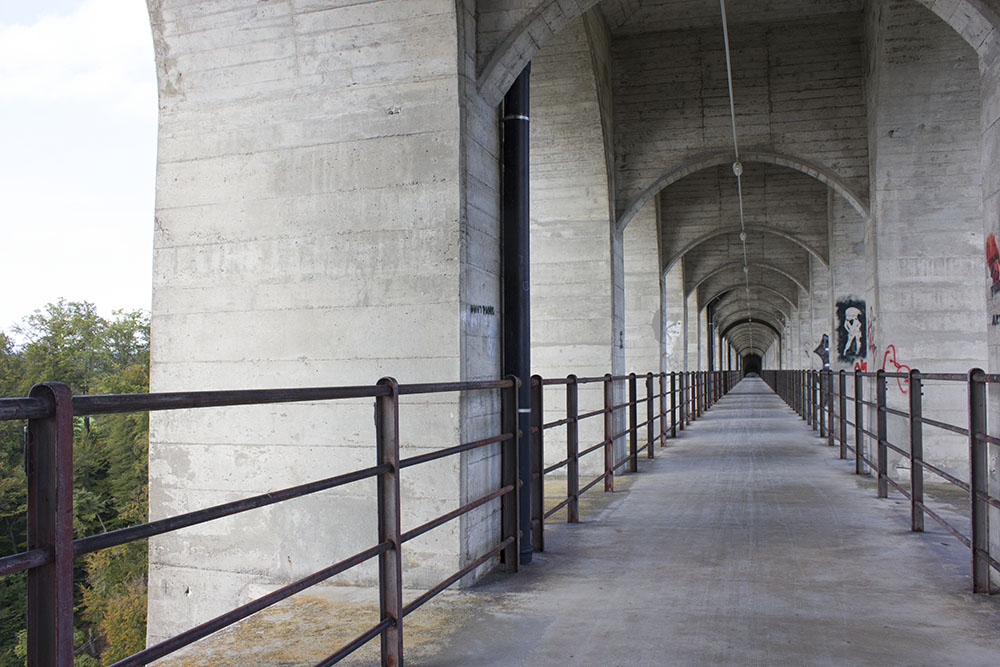
\includegraphics[width=200px]{./1_HDR/hdr/grandfey.jpg}
        \caption{The three input images (top left: normal, top right: shorter exposure, bottom left: longer exposure), and the HDR image which they produced, tonemapped with Luminance HDR and the Mantiuk'06 algorithm.}
    \end{center}
\end{figure}

\begin{figure}[htb]
    \begin{center}
        \includegraphics[width=200px]{./1_HDR/hdr/IMG_5452.jpg}
        \includegraphics[width=200px]{./1_HDR/hdr/IMG_5453.jpg}
        \includegraphics[width=200px]{./1_HDR/hdr/IMG_5454.jpg}
        \includegraphics[width=200px]{./1_HDR/hdr/poya.jpg}
        \caption{Same as above, but with the Fattal algorithm for tone mapping.}
    \end{center}
\end{figure}

\newpage
\FloatBarrier

\section{Tone Mapping using the Bilateral Filter}
\subsection*{2.2 Bilateral Filter}
Figure~\ref{img:comp} compares different parameter values for the bilateral filter on a grey-scale image. What can be clearly seen in the comparison for the parameters is that an increase in $\sigma_r$ mostly affects overall blurriness, i.e. comes closer to a ``typical'' Gaussian blur; whereas $\sigma_s$ values have an impact on the edge preserving aspect, with low values preserving the edges more strongly, and high values allowing the smoothing to occur over larger areas, ignoring more edges.
\begin{sidewaysfigure}[hp]
    \begin{center}
        \includegraphics[width=800px]{comparison.pdf}
        \caption{Comparison of different parameters for $\sigma_s$ and $\sigma_r$, inspired by the lecture slides.\label{img:comp}}
    \end{center}
\end{sidewaysfigure}

\newpage
\FloatBarrier
\subsection*{2.3 Tone Mapping using the Bilateral Filter}
The output range was set to 20 for all images.

\begin{figure}[htb]
    \begin{center}
        \includegraphics[height=250px]{bilateral_memorial.jpg}
        \includegraphics[width=300px]{bilateral_belgium.jpg}
        \caption{HDR images after tone mapping with the bilateral filter.}
    \end{center}
\end{figure}

\begin{figure}[htb]
    \begin{center}
        \includegraphics[width=400px]{bilateral_grandfey.jpg}
         \includegraphics[width=400px]{bilateral_poya.jpg}
        \caption{HDR images after tone mapping with the bilateral filter.}
    \end{center}
\end{figure}

\newpage
\FloatBarrier
\subsection*{2.5 Gaussian vs. Bilateral}
The ``simple'' Gaussian filter clearly produces halos around sharp edges, such as the fence. This effect also leads to an overall darker image, because of these pixels in the halo which are disproportionately bright. The bilateral filter, on the other hand, produces a very nice and adequate tone mapping for the HDR image.

\begin{figure}[htb]
    \begin{center}
    	\includegraphics[trim = 0px 0px 700px 0px, clip, width=200px]{bilateral_grandfey.jpg}
        \includegraphics[trim = 0px 0px 700px 0px, clip, width=200px]{gaussian_grandfey.jpg}
        \caption{Left: bilateral filter. Right: Gaussian filter. Although this is not an extreme case, we can clearly see the halos around the edges. \label{img:22zoom}}
    \end{center}
\end{figure}

\newpage
\FloatBarrier
\section{Two-Scale Photographic Tone Adjustment}
\subsection*{3.2 Different Model and Input Images}
Figure~\ref{img:nice1} and Figure~\ref{img:nice2} use a slightly modified version of the same model image, where the contrast has been reduced and the image made slightly brighter. This becomes apparent in the output, where the first version has a much higher contrast than the second. Also, the details have been scaled slightly stronger on the first image.
\begin{figure}[htb]
    \begin{center}
    	\includegraphics[width=300px]{32_nicefribourg.jpg}
    	\includegraphics[width=450px]{nicefribourg.png}
        \caption{Image \texttt{nice.jpg} as input and \texttt{fribourgbw.jpg} as model. Top: matched output, bottom: intermediate images.\label{img:nice1}}
    \end{center}
\end{figure}

\begin{figure}[htb]
    \begin{center}
    	\includegraphics[width=300px]{32_nicefribourg2.jpg}
    	\includegraphics[width=370px]{nicefribourg2.png}
        \caption{Image \texttt{nice.jpg} as input and \texttt{fribourgbw2.jpg} as model. Top: matched output, bottom: intermediate images.\label{img:nice2}}
    \end{center}
\end{figure}

\begin{figure}[htb]
    \begin{center}
    	\includegraphics[width=300px]{32_1auggrandfey.jpg}
    	\includegraphics[width=450px]{1auggrandfey.png}
    	\includegraphics[width=170px]{1auggrandfey_hist.png}
        \caption{Image \texttt{1aug.jpg} as input and \texttt{grandfey.jpg} as model. Top: matched output, middle: intermediate images, bottom: histogram of the input and model image.}
    \end{center}
\end{figure}

\begin{figure}[htb]
    \begin{center}
    	\includegraphics[width=300px]{32_grandfey1aug.jpg}
    	\includegraphics[width=450px]{grandfey1aug.png}
        \caption{Image \texttt{grandfey.jpg} as input and \texttt{1aug.jpg} as model. Top: matched output, bottom: intermediate images.}
    \end{center}
\end{figure}

\begin{figure}[htb]
    \begin{center}
    	\includegraphics[width=300px]{32_grandfeybwlily.jpg}
    	\includegraphics[width=400px]{grandfeybwlily.png}
    	\includegraphics[width=170px]{grandfeybwlily_hist.png}
        \caption{Image \texttt{grandfeybw.jpg} as input and \texttt{lily.jpg} as model. Top: matched output, middle: intermediate images, bottom: histogram of the input and model image.}
    \end{center}
\end{figure}

\begin{figure}[htb]
    \begin{center}
    	\includegraphics[width=300px]{32_lilywinterstorm.jpg}
    	\includegraphics[width=450px]{lilywinterstorm.png}
    	\includegraphics[width=170px]{lilywinterstorm_hist.png}
        \caption{Image \texttt{lily.jpg} as input and \texttt{winterstorm.png} as model. Top: matched output, middle: intermediate images, bottom: histogram of the input and model image.}
    \end{center}
\end{figure}

\FloatBarrier
\subsection*{3.3 Direct Y Channel Histogram Matching}
Observations from the direct comparison:
\begin{itemize}
\item Direct matching produces slightly blurrier images due to the lack of detail boosting. Detail is lost in histogram matching, therefore detail boosting helps in securing a sharp image.
\item Direct matching produces larger areas of one color with ``weird'' edges of the color areas (see for example in Figure~\ref{img:direct1} the van on the left or the pillars) because the details are included in the histogram.
\item As a consequence, the lack of sharp edges leads to the impression that colors are ``wrong'' (especially Figure~\ref{img:direct1}).
\end{itemize}

\begin{figure}[htb]
    \begin{center}
    	\includegraphics[width=220px]{32_nicefribourg.jpg}
    	\includegraphics[width=220px]{33_nicefribourgbw.jpg}
        \caption{Image \texttt{nice.jpg} as input and \texttt{fribourgbw.jpg} as model. On the left, the image from section 3.2; on the right, the image after direct histogram mapping.\label{img:direct1}}
    \end{center}
\end{figure}

\begin{figure}[htb]
    \begin{center}
    	\includegraphics[width=220px]{32_grandfeybwlily.jpg}
    	\includegraphics[width=220px]{33_grandfeybwlily.jpg}
        \caption{Image \texttt{grandfeybw.jpg} as input and \texttt{lily.jpg} as model. On the left, the image from section 3.2; on the right, the image after direct histogram mapping.\label{img:direct2}}
    \end{center}
\end{figure}

\begin{figure}[htb]
    \begin{center}
    	\includegraphics[width=220px]{32_lilywinterstorm.jpg}
    	\includegraphics[width=220px]{33_lilywinterstorm.jpg}
        \caption{Image \texttt{lily.jpg} as input and \texttt{winterstorm.png} as model. On the left, the image from section 3.2; on the right, the image after direct histogram mapping.\label{img:direct3}}
    \end{center}
\end{figure}






\newpage
\FloatBarrier
\section{Bonus}
\subsection*{Interesting Model Histograms}

I have created two different models with interesting histograms with photoshop. The first is a simple gradient which reaches from a dark grey to a very light grey, black and white are not present. Also, the dark part at the beginning and the light part in the end are present in more pixels than the value inbetween. Since the model image is only 75 pixels wide, it will in a way flatten images that are mapped to it.

The second is an image of RGB and CMY colors, where the luminance values are mostly in a narrow middle area of the histogram. This will reduce the contrast in matched images.
\begin{figure}[h]
    \begin{center}
    	
\includegraphics[width=150px]{model_gradient.png}
    	\includegraphics[width=160px]{hist_gradient.png}\\
    	
\includegraphics[width=80px]{model_rgbcmy.png}\hspace{70px}
    	\includegraphics[width=160px]{hist_rgbcmy.png}
        \caption{Model images and their respective histograms.}
    \end{center}
\end{figure}

Here are a couple of images where these models were applied using the \texttt{autoToneAdj} function, also with different detail scaling factors.

\begin{figure}[h]
    \begin{center}
    	\includegraphics[width=220px]{bonus_1aug.jpg}
    	\includegraphics[width=220px]{1aug_gradient_3.jpg}
    	\includegraphics[width=220px]{1aug_rgbcmy_2.jpg}
    	\includegraphics[width=220px]{1aug_rgbcmy_4.jpg}
        \caption{Clockwise from top left: original, gradient, detail*3; rgbcmy, detail*4; rgbcmy, detail*2.}
    \end{center}
\end{figure}

\begin{figure}[h]
    \begin{center}
    	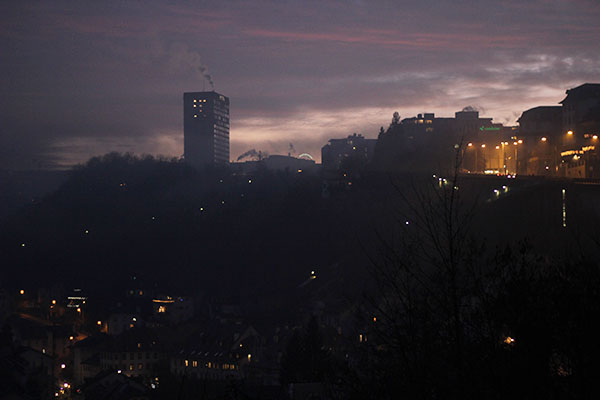
\includegraphics[width=300px]{bonus_fribourg.jpg}
    	\includegraphics[width=300px]{fribourg_gradient_6.jpg}
    	\includegraphics[width=300px]{fribourg_rgbcmy_4.jpg}
        \caption{Top to bottom: original, gradient, detail*6; rgbcmy, detail*4.}
    \end{center}
\end{figure}

\begin{figure}[h]
    \begin{center}
    	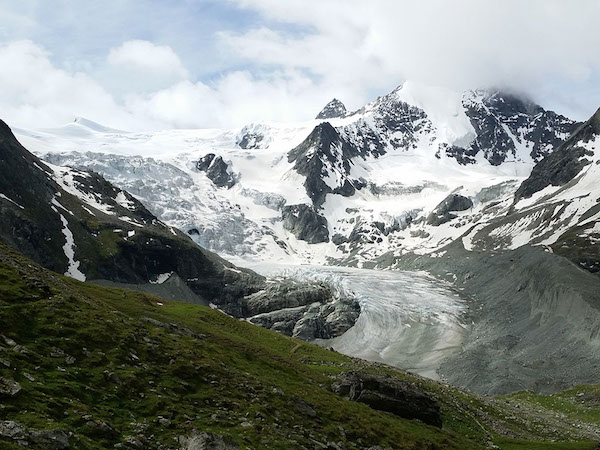
\includegraphics[width=270px]{bonus_moiry.jpg}
    	\includegraphics[width=270px]{moiry_gradient_06.jpg}
    	\includegraphics[width=270px]{moiry_rgbcmy_4.jpg}
        \caption{Top to bottom: original, gradient, detail*0.6; rgbcmy, detail*4.}
    \end{center}
\end{figure}

\begin{figure}[h]
    \begin{center}
    	\includegraphics[width=220px]{bonus_nice.jpg}
    	\includegraphics[width=220px]{nice_gradient_5.jpg}
    	\includegraphics[width=220px]{nice_rgbcmy_05.jpg}
    	\includegraphics[width=220px]{nice_rgbcmy_6.jpg}
        \caption{Clockwise from top left: original, gradient, detail*5; rgbcmy, detail*6; rgbcmy, detail*0.5.}
    \end{center}
\end{figure}

\begin{figure}[h]
    \begin{center}
    	\includegraphics[width=220px]{bonus_stjean.jpg}
    	\includegraphics[width=220px]{stjean_gradient_03.jpg}
    	\includegraphics[width=220px]{stjean_gradient_4.jpg}
    	\includegraphics[width=220px]{stjean_rgbcmy_15.jpg}
        \caption{Clockwise from top left: original, gradient, detail*0.3; rgbcmy, detail*1.5; gradient, detail*4.}
    \end{center}
\end{figure}


\newpage
\FloatBarrier
\subsection*{RGB channel-wise histogram matching}
This method produces interesting results where, unlike the direct matching or the tone adjustment with two-scale decomposition and detail enhancement, the contrast is not the main aspect that is affected by the matching, but also the color distribution. If the color channels are nicely distributed, this can produce interesting results. However, the colors will of course appear to be slightly unrealistic when matching from another image.

Matching with greyscale images will, as before, impact the contrast and not the colors, because the 3 histograms for R, G and B are identical.

\begin{figure}[htb]
    \begin{center}
    	\includegraphics[width=220px]{nice_fbw_chan.jpg}
        \includegraphics[width=220px]{nice_rgbcmy_chan.jpg}
        \caption{Image \texttt{nice.jpg} matched with \texttt{fribourgbw.jpg} (left) and \texttt{model\_rgbcmy.png} (right).}
    \end{center}
\end{figure}

\begin{figure}[htb]
    \begin{center}
    	\includegraphics[width=220px]{lily_wi_chan.jpg}
        \includegraphics[width=220px]{lily_rgbcmy_chan.jpg}
        \caption{Image \texttt{lily.jpg} matched with \texttt{winterstorm.png} (left) and \texttt{model\_rgbcmy.png} (right).}
    \end{center}
\end{figure}

%-------------------------
\end{document}
%-------------------------







